L’architettura di Nexify utilizzerà la struttura a microservizi in quanto ci permette di realizzare un’architettura che scala e che permette di variare la potenza e le risorse assegnate ad ogni microservizio.\\
Inoltre porta un grande vantaggio in termini di deployment e developement in quanto permette l’assegnazione di ogni microservizio a piccoli team indipendenti (“two pizzas” team), facilita il coinvolgimento di nuovo personale e permette di scomporre l’applicativo monolitico in tanti semplici e più facilmente gestibili servizi. Per questi motivi sono facilitati il testing e la continua integrazione.\\
Per la suddivisione del software in microservizi utilizziamo in pattern Decompose by subdomains che ci permette di assegnare un microservizio ad ogni sottodominio che comprende azioni tutte strettamente legate fra loro (così da evitare accoppiamento).\\
La memoria persistente (database) verranno gestiti secondo il pattern Database per Service, che prevede l’utilizzo di un database per ogni servizio, cosi da rendere il servizio completamente indipendente dal resto del software. La distribuzione del database verrà gestita tramite il pattern Saga in modalità Choreography per la corretta esecuzione delle transazioni.\\
L’accesso ai servizi sarà garantito attraverso un API Gateway che interagisce con i singoli servizi attraverso delle API REST. Ogni tipo di client (Web o Desktop) si interfaccerà con il proprio API Gateway.\\
\begin{figure}[!h]
\centering
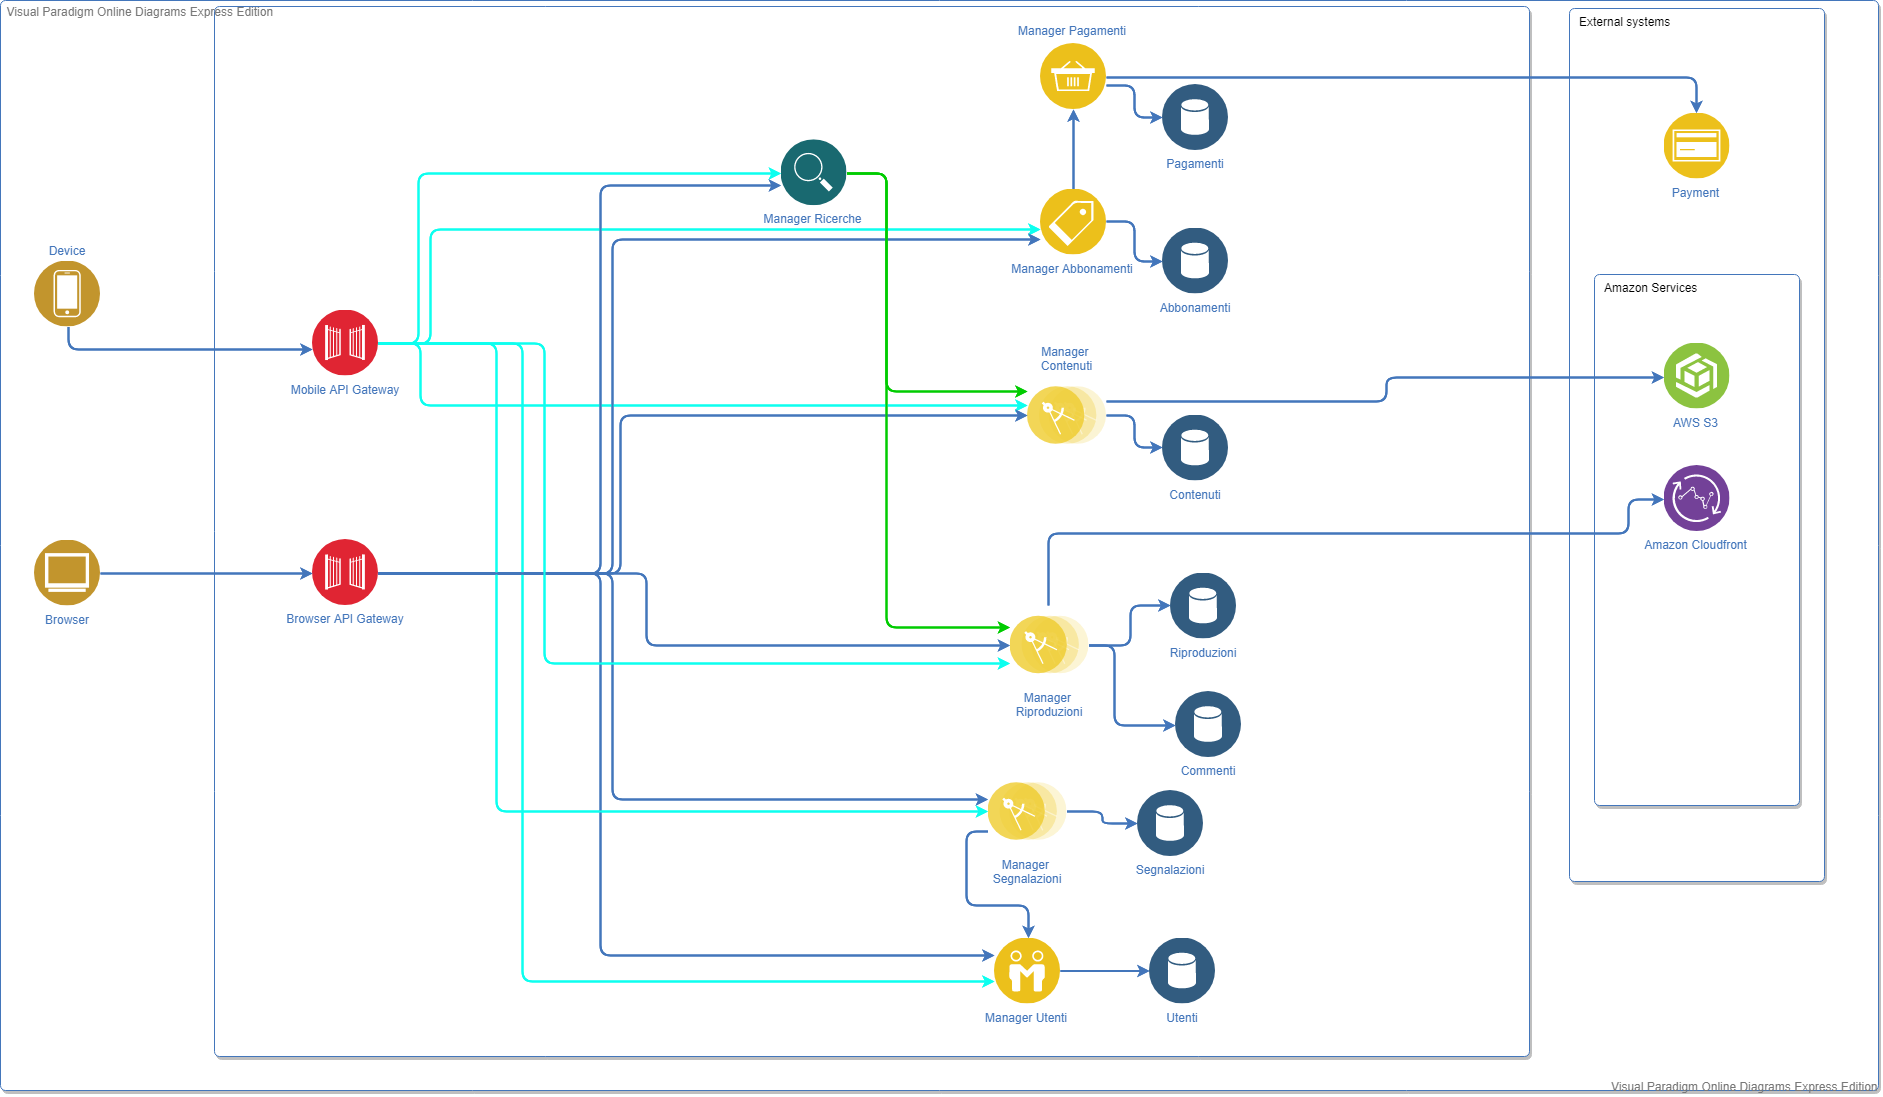
\includegraphics[scale=0.24]{../Contents/Diagrams/Design/architecture/Architecture.png}
\end{figure}
\subsection{Implementazione microservizi}
Potenzialmente è possibile usare tecnologie diverse per ciascun microservizio (questo è un altro vantaggio di quest'architettura), nel nostro caso si è però scelto di utilizzare Django per l'implementazione di ciascun microservizio. Questo perché Django è stato ritenuto adatto a tutte le funzionalità da implementare e non si avrebbero grandi benefici a differenziare le tecnologie in questo caso. Django è un framework basato su python, contenente svariati moduli per la gestione di task ricorrenti nella programmazione web. La comunicazione tra gli elementi di frontend e Django avviene tramite protocollo https, nelle request verrà sempre inviato un oggetto di session per ottenere dati sull'utente.
\subsubsection{Django authentication system}
Uno dei moduli di django è django.contrib.auth che consente di gestire l'autenticazione degli utenti. La classe di default per rappresentare l'account di un utente è User, ma si possono facilmente definire account custom ereditando dalla classe AbstractBaseUser, e nel nostro caso verrà seguita questa strategia in modo da creare un Account secondo le esigenze di Nexify. Il modulo mette poi a disposizione le funzioni:
\begin{itemize}
\item authenticate($<$username$>$, $<$password$>$), che verifica la presenza di un account con le credenziali fornite ed eventualmente lo restituisce (restituisce None altrimenti). Si occupa quindi anche di interfacciarsi al database degli account, e inoltre effettua l'hashing delle password. Notiamo infatti che le password vengono inviate non hashate, ma non si creano problemi di sicurezza in quanto viene utilizzato il protocollo https che si occupa di criptare i pacchetti. 
\item login($<$session$>$, $<$account$>$) che viene usato per collegare l'id dell'account alla sessione dell'utente, in modo da poter ottenere l'account dell'utente in seguito a request successive (l'account sarà infatti ottenibile con con request.user)
\item logout($<$session$>$) che viene usato per scollegare la sessione dell'utente dall'account
\end{itemize}
\subsection{Databases}
Verranno usati database relazionali per i database:
\begin{itemize}
\item Utenti
\item Abbonamenti
\item CodaDiRiproduzione
\end{itemize}
mentre si useranno database nosql per i database:
\begin{itemize}
\item Sottoscrizioni
\item Contenuti
\item Commenti
\item Riproduzioni
\end{itemize}
in quanto ci si aspetta una grande quantità di commenti, riproduzioni, sottoscrizioni ad abbonamenti e contenuti. Come database relazione verrà usato PostgreSQL, mentre come non relazionale si userà MongoDB. Django permette di accedere a database relazioni tramite ORM, quindi sostanzialmente si possono fare query al database in uno stile Object Oriented. Inoltre usando l'estensione Django-MongoDB-engine è possibile accedere a database nosql in maniera pressoché identica a come si fa con un ORM (ci sono alcune funzionalità che non saranno disponibili ma di cui non faremo uso). Guardare la sezione sui diagrammi di sequenza per un maggiore approfondimento sull'accesso ai database.
\subsection{Pattern DAO}
Nonostante Django abbia molti moduli standard che permettono un'astrazione dal database (come nel caso dell'autenticazione, in cui è Django a interfacciarsi col database), in molti casi sarà necessario interfacciarsi ai vari database. Si è quindi deciso di adottare il pattern DAO (data access object), che permette di separare l'accesso ai dati a basso livello da richieste ad alto livello per ricevere dati, è infatti implementato, in generale, mediante due classi:
\begin{itemize}
\item la classe DAO, che si occupa di interfacciarsi con la sorgente di dati a basso livello (nel nostro caso si tratterà principalmente di database), consentendo quindi alle altre classi di effettuare query senza conoscere dettagli di implementazione a basso livello
\item una classe tipicamente chiamata ValueObject che contiene i dati ricavati dalla classe DAO e viene fornita come risultato alle classi che fanno richieste a DAO.
\end{itemize}
La scelta di adottare DAO è stata anche dettata dal fatto che, nonostante utilizzeremo Django per tutti i microservizi, l'accesso a database relazionali è diverso dall'accesso a database nosql, e quindi attraverso DAO si possono fare richieste senza preoccuparsi dell'eterogeneità dei database.
\subsection{CDN}
Per la CDN è stato scelto Amazon CloudFront, che ha dimostrato con altre piattaforme di essere in grado di scalare a livello mondiale e fornisce costi che dipendono dal consumo effettuato. In realtà CloudFront sarà affiancato da altri servizi Amazon, e in particolare verrà adottata l'architettura di video streaming on demand proposta da Amazon:\\
\begin{figure}[!h]
\centering
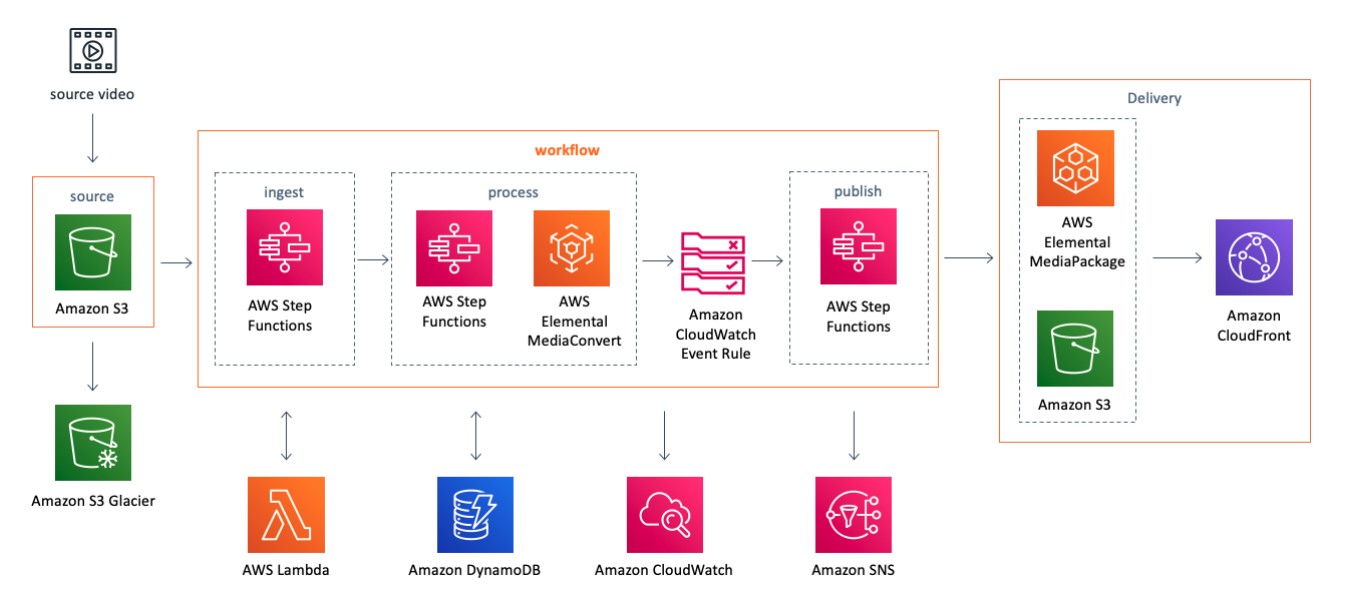
\includegraphics[scale=0.45]{aws_ondemand_streaming.png}
\end{figure}\\
Quando un utente carica un video, questo viene memorizzato usando Amazon S3, che è un servizio di storage di oggetti. Si entra poi in una fase di ingest in cui vengono fatti controlli sul corretto caricamento del file, sul formato del file e controlli simili; una volta superati questi controlli si entra nella fase di process in cui si creano varie versioni del video codificate in formati diversi in modo da garantire la disponibilità su una vasta gamma di dispositivi, le versioni avranno anche bitrate diversi in modo da poter effettuare uno streaming adattivo. Viene poi genarato un URL per il video su S3 e CloudFront (usando le AWS Step Functions), con il quale è possibile accedere al video. L'architettura fornisce anche altre funzionalità, come Simple Notification Service che invia notifiche all'amministratore in casi di errore, il database Dynamo viene usato, tra le altre cose, per tenere un log delle operazioni eseguite nell'infrastruttura. CloudFront è la CDN vera e propria, a cui gli utenti faranno richieste per ricevere video in streaming. Va sottolineato che il solo evento di caricamento su S3 è un trigger che fa partire l'intero workflow fino alla generazione degli URL CloudFront. Inoltre anche il video originale può essere mantenuto su S3, e questo sarà utile per poterlo eventualmente scaricare. Un altro aspetto da notare è che gli oggetti salvati su S3 sono divisi in bucket, e ogni bucket è localizzato in una singola regione del mondo; si possono però creare più bucket distribuiti in più regioni e usando il Cross-Region-Replication implementato da Amazon, è possibile replicare le risorse di un bucket su tutti gli altri distribuiti nelle altre regioni; dal punto di vista di CloudFront questo non crea problemi, in quanto CloudFront può gestire più origins (cioè le locazioni dei bucket da cui prendere le risorse).\\
Una volta configurata quest'architettura mediante la console di Amazon, sarà sufficiente usare S3 per caricare risorse e CloudFront per ricevere streaming di risorse. \'E da notare che gli utenti in realtà caricheranno i file prima su django, e poi django penserà a caricarli su S3, dopo averli opportunamente fusi insieme, questo può comportare dei ritardi extra nel caricamento delle risorse (in quanto è necessario fare l'upload in realtà 2 volte), però è necessario sia per motivi di sicurezza: non si vuole fornire accesso diretto ad AWS agli utenti, sia per alleggerire il carico di lavoro sui dispositivi degli utenti, in quanto la fusione viene effettuata da django.
\subsubsection{MKV}
I file caricati su S3 saranno file MKV: gli utenti potranno caricare singoli file che saranno poi uniti in un singolo file MKV. Per effettuare questa fusione verrà usato pymkv, un wrapper python che consente di usare tool di MKVToolNix. In particolare le funzioni messe a disposizione sono:
\begin{itemize}
\item add\_track(pathIn) che consente di aggiungere una traccia video/audio o un file sottotitoli
\item mux(pathOut) che consente di fondere le tracce aggiunte in un unico file MKV
\end{itemize}
\subsubsection{CloudFront Signed URLs}
L'accesso a un URL CloudFront associato a una risorsa verrà negato agli utenti, in quanto chiunque dovesse riuscire ad avere tale URL potrebbe altrimenti accedere alla risorsa, anche non passando attraverso la piattaforma. Per assicurarci che le richieste a CloudFront arrivino da Nexify, si utilizzeranno i signed URLs messi a disposizione da CloudFront: partendo dall'URL CloudFront della risorsa, si genera un altro URL firmato e che contiene una politica di accesso. Nella politica è possibile specificare gli indirizzi IP che possono accedere all'URL e per quanto tempo è possibile accedere a tale URL. Visto che gli URL verranno firmati con una chiave privata di Nexify, questo ci assicurerà che per ottenere degli URL accessibili si sia passati attraverso la piattaforma.
\subsection{FrontEnd}
La piattaforma sarà disponibile sia in versione web che mobile, il backend sarà ovviamente comune a tali versioni, mentre il frontend web verrà realizzato con ReactJS e Bootstrap, mentre il frontend mobile attraverso Flutter. Alcune classi del backend saranno presenti anche nel frontend (o meglio, nel frontend avremo una classe corrispondente, visto che i linguaggi di frontend e backend sono diversi), in modo da poter salvare più agevolmente risultati di richieste, e lavorare con la stessa struttura dei dati.
\subsection{Diagramma delle classi design}
Nella cartella ``Diagrams/Design/class" sono riportati i diagrammi delle classi di design. In ``Diagrams/Design/class/Entity" vengono mostrate tutte le entità e le loro relazioni che non verranno quindi riportate negli altri diagrammi. In ``Diagrams/Design/class/Package" vengono mostrate le dipendenze tra i vari package, mentre tutti gli altri diagrammi si concentrano sulle classi contenute in singoli package.
\subsection{Diagrammi di Sequenza}
Nella cartella ``Diagrams/Design/sequence'' sono riportati i diagrammi di sequenza di design, che sono il raffinamento, in seguito alla scelta della tecnologia, dei corrispettivi diagrammi di analisi.\\
Nei diagrammi, per non appesantirli troppo, non saranno mostrate le interazioni tra le classi DAO ed i database (quando opportuno, sarà però mostrata la generazione dei risultati delle query). Mostriamo però qui degli esempi di query/insert/update/delete generici, le operazioni richieste negli altri diagrammi di sequenza saranno quindi facilmente derivabili. Sono mostrate, in ordine, le operazioni di create, query, update e delete. I diagrammi sono essenzialmente uguali anche per i database nosql, e quindi non vengono mostrati.\\
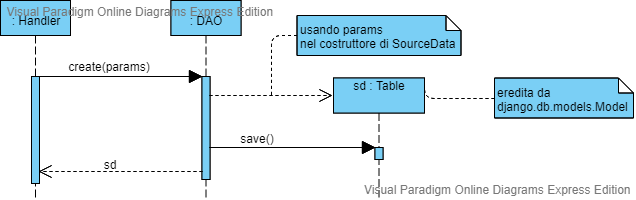
\includegraphics[scale=0.7]{../Contents/Diagrams/Design/sequence/DAO/create.png}\\ \\
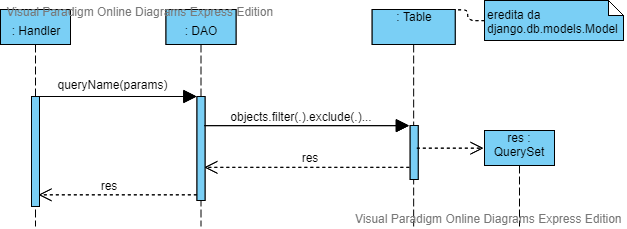
\includegraphics[scale=0.7]{../Contents/Diagrams/Design/sequence/DAO/query.png}\\ \\
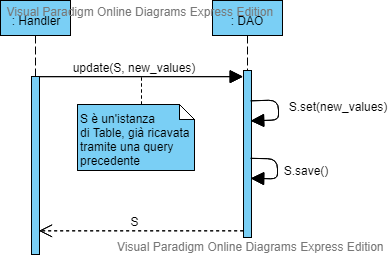
\includegraphics[scale=0.7]{../Contents/Diagrams/Design/sequence/DAO/update.png}\\ \\
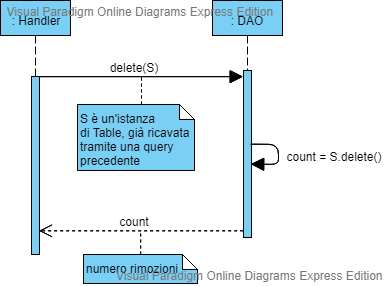
\includegraphics[scale=0.7]{../Contents/Diagrams/Design/sequence/DAO/delete.png}\\
Alcuni diagrammi di sequenza di analisi, in design si traducono in delle query, e di conseguenza non verrà mostrato il diagramma di design corrispondente. Tali diagrammi sono:
\begin{itemize}
\item RecuperaAbbonamentiEsistenti
\item RecuperaAbbonamentiUtente
\item RecuperaProdottiUtente
\item RecuperaServizi
\item RecuperaServiziAbbonamento
\end{itemize}
mostriamo quindi qui, per completezza, l'implementazione di queste query:
\begin{itemize}
\item PianoDiAbbonamento.objects.all()
\item SottoscrizioneAbbonamento.objects.filter(account=Acc).filter(F(data)+F(piano\_\_durata)\_\_gt=now())
\item Prodotto.objects.filter(proprietario=Acc)
\item Servizio.objects.all()
\item PianoServizioRelationship.objects.filter(piano=P)
\end{itemize}
Sono state scritte solo le query vere e proprie, che vanno immaginate nel contesto del diagramma generico per le query. Per effettuare le proiezioni verranno restituiti da DAO solo i campi necessari.
\newline\newline
\noindent{\large \textbf{Revisioni 11}} \\ \\
\begin{tabular}{|c | c | c | c|} 
 	\hline
	 Numero & Data & Descrizione \\ [0.5ex] 
	\hline\hline
	1 & 20/04/2020 & Stesura iniziale \\ 
	\hline
	2 & 08/05/2020 & Scelta di Django come tecnologia \\
	\hline
\end{tabular}